\documentclass[11pt]{scrartcl}
\usepackage[utf8]{inputenc}
\usepackage{mathtools}
\usepackage{amssymb}

\usepackage{caption}
\usepackage{color}
\usepackage{xcolor}
\usepackage{listings}
\DeclareCaptionFont{white}{\color{white}}
\DeclareCaptionFormat{listing}{\colorbox{gray}{\parbox{\textwidth}{#1#2#3}}}
\captionsetup[lstlisting]{format=listing,labelfont=white,textfont=white}

\usepackage{tikz}
\usetikzlibrary{automata,positioning}


\title{\textbf{1810 Einsendeaufgabe KE 01}}
\author{Gustavo Nunes Martins}

\begin{document}
	\maketitle
	\section*{Aufgabe 1}
	\subsubsection*{a-1}
	\textbf{Falsch}. Laut "Hopcroft: Introduction to Automata Theory, Languages and Computation 2er Ausgabe, Seite 30":
	
	\begin{center}
		$\varSigma^{*}=\varSigma^{0}\bigcup\varSigma^{1}\bigcup\varSigma^{2}\bigcup...$
	\end{center}
	
	Es gilt deshalb $\varSigma^{*}=\{\varepsilon\}=\varSigma^{0}$ nur wenn $\varSigma^{1}\bigcup\varSigma^{2}\bigcup...=\emptyset\Rightarrow\varSigma^{1}=\varSigma=\emptyset$, also nur wenn die Alphabet eine leere Menge ist. 
	
	Das widerspricht die Definition von Alphabet (gleiches Buch, Seite 28), wobei eine Alphabet keine leere Menge sein darf.
	\subsubsection*{a-2}
	\textbf{Falsch}, denn jeder regulären Ausdruck hat eine entsprechende endlicher Automat (diese Prozess kann automatisch durchgeführt werden durch den Thompson Algorithmus)
	\subsection*{b}
	\textbf{TODO}
	\subsection*{c}
	$L=\{w\in\{0,1\}^{*}|$ die Mindestlänge von w ist 3 und endet nicht mit 111\}
	\subsection*{d}
	Der Minimalfall trifft zu wenn alle Symbolen eines Wortes \textbf{gleich} sind (die String ist der form a...a). Dann gilt es:
	\begin{itemize}
		\item Teilworter Länge 1: \{a\} (1 Teilwort)
		\item Teilworter Länge 2: \{aa\} (1 Teilwort)
		\item Teilworter Länge 3: \{ aaa\} (1 Teilwort)
		\item Teilworter Länge n: \{ aaa...\} (1 Teilwort)
		\item Alle Teilworter von lange 1 bis n: \{a,aa,aaa,aaa...\}. (n Teilwörter)
		\item 	Total: \textbf{n} distinkte Teilwörter für das Minimalfall
	\end{itemize}
	Der Minimalfall trifft zu wenn alle Symbolen eines Wortes \textbf{anders} sind (die String ist der Form abcdef...). Dan gilt es:
	\begin{itemize}
		\item Teilworter Länge 1: \{a,b,c,d,e,f,...\} (n Teilwörter)
		\item Teilworter Länge 2: \{ab,bc,cd,ef,f...,...\} (n-1 Teilwörter)
		\item Teilworter Länge 3: \{ abc,bcd,cde,def,ef...,f...,...\} (n-1 Teilwörter)
		\item Teilworter Länge n: \{ abcdef......\} (1 Teilwort)
		\item Alle Teilworter von lange 1 bis n: n+(n-1)+(n-2)+(n-3)+...+1=(n+1)*n/2. 
		\item 	Total: \textbf{(n+1)*n/2} distinkte Teilwörter für das Maximalfall
	\end{itemize}
	\subsection*{e}
	\textbf{TODO}
	\subsection*{f}
	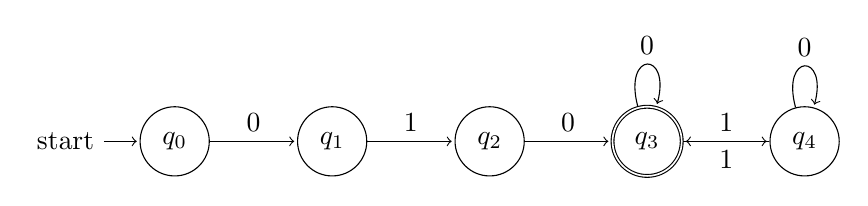
\begin{tikzpicture}[shorten >=1pt,node distance=2cm,on grid,auto] 
	\node[state,initial] (q_0)   {$q_0$}; 
	\node[state] (q_1) [right=of q_0] {$q_1$}; 
	\node[state] (q_2) [right=of q_1] {$q_2$}; 
	\node[state,accepting](q_3) [right=of q_2] {$q_3$};	\node[state] (q_4) [right=of q_3] {$q_4$};

	\path[->] 
	(q_0) edge  node {0} (q_1)
	(q_1) edge  node  {1} (q_2)
	(q_3) edge [loop above] node {0} ()
	(q_2) edge  node {0} (q_3) 
	(q_3) edge node {1} (q_4) 
	(q_4) edge  node {1} (q_3) 
	(q_4) edge [loop above] node{0} ()
	;
	\end{tikzpicture}
	\section*{Aufgabe 2}	\begin{lstlisting}[label=some-code,caption=Lexer Code f\"{u}r das REAL token,language=C]
#define TRUE 1

int gettoken(){
int c;
state = 0; start_state=0;
	
while (TRUE){
switch(state){
case 11:
	c = nextchar();
	if isdigit(c)		state=12;
	else if issign(c)	state=13;
	else			state=next_diagram();
	break;

case 12:
	c = nextchar();
	if c=='.'		state=14;
	else if isdigit(c)	state=12;
	else			state=next_diagram();
	break;

case 13:
	c=nextchar();
	if isdigit(c)		state=12;
	else			state=next_diagram();
	break;

case 14:
	c=nextchar();
	if isdigit(c)		state=15;
	else if c=='E'		state=17;
	else			state=16;
	break;

case 15:
	c=nextchar();
	if isdigit(c)		state=15;
	else if c=='E'		state=17;
	else			state=16;
	break;
	
case 16:
	return REAL;
	break;
	
case 17:
	c=nextchar();
	if isdigit(c)		state=18;
	else if issign(c)	state=19;
	else			state=next_diagram();
	break;
	
case 18;
	c=nextchar(c)
	if isdigit(c)		state=18;
	else			state=16;
	break;
	
case 19:
	c=nextchar();
	if isdigit(c)		state=18;
	else			state=next_diagram();
}
}
}
	\end{lstlisting}
	\section*{Aufgabe 3}
	Anmerkungen: 
	\begin{itemize}
		\item Das lesen von negativ-Nummern lauft nicht nur durch den Lexer, aber auch durch den Parser. Das erleichtert die Entscheidung von "-" als negativ-Nummern oder als Subtraktion.
		\item Punkte (z.B. (3,2) oder (p,5)) und Funktionen ((v, f(v)) sind alle durch Tupeln repr\"{a}sentiert.
		\item Relative Bindungskräfte zwischen Multiplikation, Division, Summierung und Subtraktion sind durch \%token Vorrang verwirklicht:
		\begin{verbatim}
		%left '+' '-'
		%left '*' '/' "mod"
		\end{verbatim}
		\item Funktionen sind entweder in Prefix- (setcolor, arc, plot usw) oder Infixform (+, -, mod usw). Alle prefix Funktionen sind durch eine IDENTIFIER RIGHTPARENTHESIS identifiziert (die Programm kann sehr einfach mit extra Funktionen erweitert werden). Infix-Funktionen sind einzeln implementiert
		\item Der Bison und FLex Code fürs Lexer und Parser ist als zip Datei geliefert.
	\end{itemize}\begin{flushleft}
	\subsection*{program}
		\includegraphics[width=1\linewidth]{../../../../Desktop/ui/diagram/program}
		\begin{verbatim}
		program  ::= PICTURE VAL_STRING declarations START commands END
		\end{verbatim}
	\subsection*{declarations}
		\includegraphics[width=0.45\linewidth]{../../../../Desktop/ui/diagram/declarations}
		\begin{verbatim}
		declarations ::= empty
							| declarations declaration
		\end{verbatim}
	\subsection*{declaration}
		\includegraphics[width=0.45\linewidth]{../../../../Desktop/ui/diagram/declaration}
		\begin{verbatim}
		declaration ::= VAR list ':' TYPE ';'
		\end{verbatim}
		\subsection*{commands}
		\includegraphics[width=0.45\linewidth]{../../../../Desktop/ui/diagram/commands}
		
		\begin{verbatim}
		
		commands ::= empty
		| commands command
		\end{verbatim}
			\subsection*{command}
		\includegraphics[width=0.45\linewidth]{../../../../Desktop/ui/diagram/command}
		\begin{verbatim}
		command  ::= assign ';'
		| fcall ';'
		| loop ';'
		| IDENTIFIER ';'
		\end{verbatim}
			\subsection*{assign}
		\includegraphics[width=0.60\linewidth]{../../../../Desktop/ui/diagram/assign}
		\begin{verbatim}
		assign   ::= IDENTIFIER ':=' potentialvalue
		| IDENTIFIER '<-' potentialvalue
		\end{verbatim}
			\subsection*{fcall}
		\includegraphics[width=0.60\linewidth]{../../../../Desktop/ui/diagram/fcall}\begin{verbatim}
		fcall    ::= FCALLPREFIXOPEN list ')'
		| fcall_nonprefix
		\end{verbatim}
			\subsection*{loop}
		\includegraphics[width=1\linewidth]{../../../../Desktop/ui/diagram/loop}
		\begin{verbatim}
		loop     ::= FOR IDENTIFIER ':=' potentialvalue TO potentialvalue STEP potentialvalue DO commands DONE
		\end{verbatim}
			\subsection*{potentialvalue}
		\includegraphics[width=0.45\linewidth]{../../../../Desktop/ui/diagram/potentialvalue}
		\begin{verbatim}
		potentialvalue
		::= value
		| IDENTIFIER
		| fcall
		| '<<' list '>>'
		| '{' commands '}'
		| '(' potentialvalue ')'
		\end{verbatim}
			\subsection*{list}
		\includegraphics[width=0.45\linewidth]{../../../../Desktop/ui/diagram/list}
		\begin{verbatim}
		list     ::= potentialvalue
		| list ',' potentialvalue
		\end{verbatim}
			\subsection*{fcall\_nonprefix}
		\includegraphics[width=0.45\linewidth]{../../../../Desktop/ui/diagram/fcall_nonprefix}
		\begin{verbatim}
		fcall_nonprefix
		::= potentialvalue '+' potentialvalue
		| potentialvalue '-' potentialvalue
		| potentialvalue '*' potentialvalue
		| potentialvalue '/' potentialvalue
		| potentialvalue 'mod' potentialvalue
		| '+' potentialvalue
		| '-' potentialvalue
		\end{verbatim}
			\subsection*{value}
		\includegraphics[width=0.45\linewidth]{../../../../Desktop/ui/diagram/value}
		\begin{verbatim}
		value    ::= '(' potentialvalue ',' potentialvalue ')'
		| VAL_INT
		| VAL_NUM
		| VAL_STRING
		\end{verbatim}
\end{flushleft}

	
\end{document}